%========================================================================
% Modelo para elaboracao de textos academicos: TCC, dissertacoes e teses
% Elaborado pelo GISIS - Grupo de Imageamento Sismico e Inversão Sismica.
%========================================================================
\chapter{Revisão Bibliográfica}
\label{ch:revisaobibliografica}

A modelagem e tomografia sísmica são técnicas essenciais na exploração de recursos naturais subterrâneos e na caracterização da subsuperfície terrestre. A tomografia sísmica é um método não invasivo que permite mapear as propriedades físicas do subsolo através da análise das ondas sísmicas geradas por fontes controladas. Um dos principais desafios na tomografia sísmica é a obtenção de informações precisas sobre as trajetórias das ondas sísmicas e suas velocidades de propagação em diferentes camadas geológicas. Nesse sentido, a equação \textit{eikonal}  é uma ferramenta fundamental para a modelagem e inversão e imageamento sísmico, pois descreve as frentes de onda e permite calcular os tempos de percurso das ondas sísmicas. Neste capítulo é explorado a equação eikonal, três resoluções numéricas e sua aplicação na tomografia de refração. Ao explorar esses tópicos, este capítulo fornecerá abrangentes conceitos utilizados na geração dos resultados deste trabalho.

\section{Modelagem sísmica}

equação analítica; limitações

equações numéricas;
	
frente de onda completa (complexidade do meio)
	
simplificação da primeira chegada (limitações do meio)

\cite{rosa2010analise}
\cite{sheriff1995exploration}




\subsection*{Equação da onda para meios acústicos}

equação completa

resolução por diferenças finitas

\cite{igel2017computational}





\subsection*{Equação analítica para ondas refratadas}

livro do kearey \cite{kearey2002introduction}






\subsection*{Equação \textit{eikonal}}

partir da equação da onda em meios acústicos

\cite{cerveny2003seismic}
\cite{rawlinson2008seismic}

eikonal e transporte





\subsection*{Método clássico}

\cite{vidale1988finite}
\cite{podvin1991finite}
\cite{afnimar2000finite}
\cite{tryggvason2006travel}

desenvolvimento com o algoritmo time3d








\subsection*{\textit{Fast Iterative Method}}

\cite{jeong2008fast}
\cite{sethian1999fast}

\cite{fu2011fast, fu2013fast}

\cite{dang2014fast, hong2016multi, hong2022mg}

\cite{cai2023improved}

desenvolvimento com a implementação 






\subsection*{\textit{Fast Sweeping Method}}

original fast sweeping method

\cite{zhao2005fast}

\cite{zhao2007parallel}

\cite{detrixhe2013parallel}

\cite{noble2014accurate}


\subsection*{Comparação numérica}


\begin{figure}[H]
	\centering
	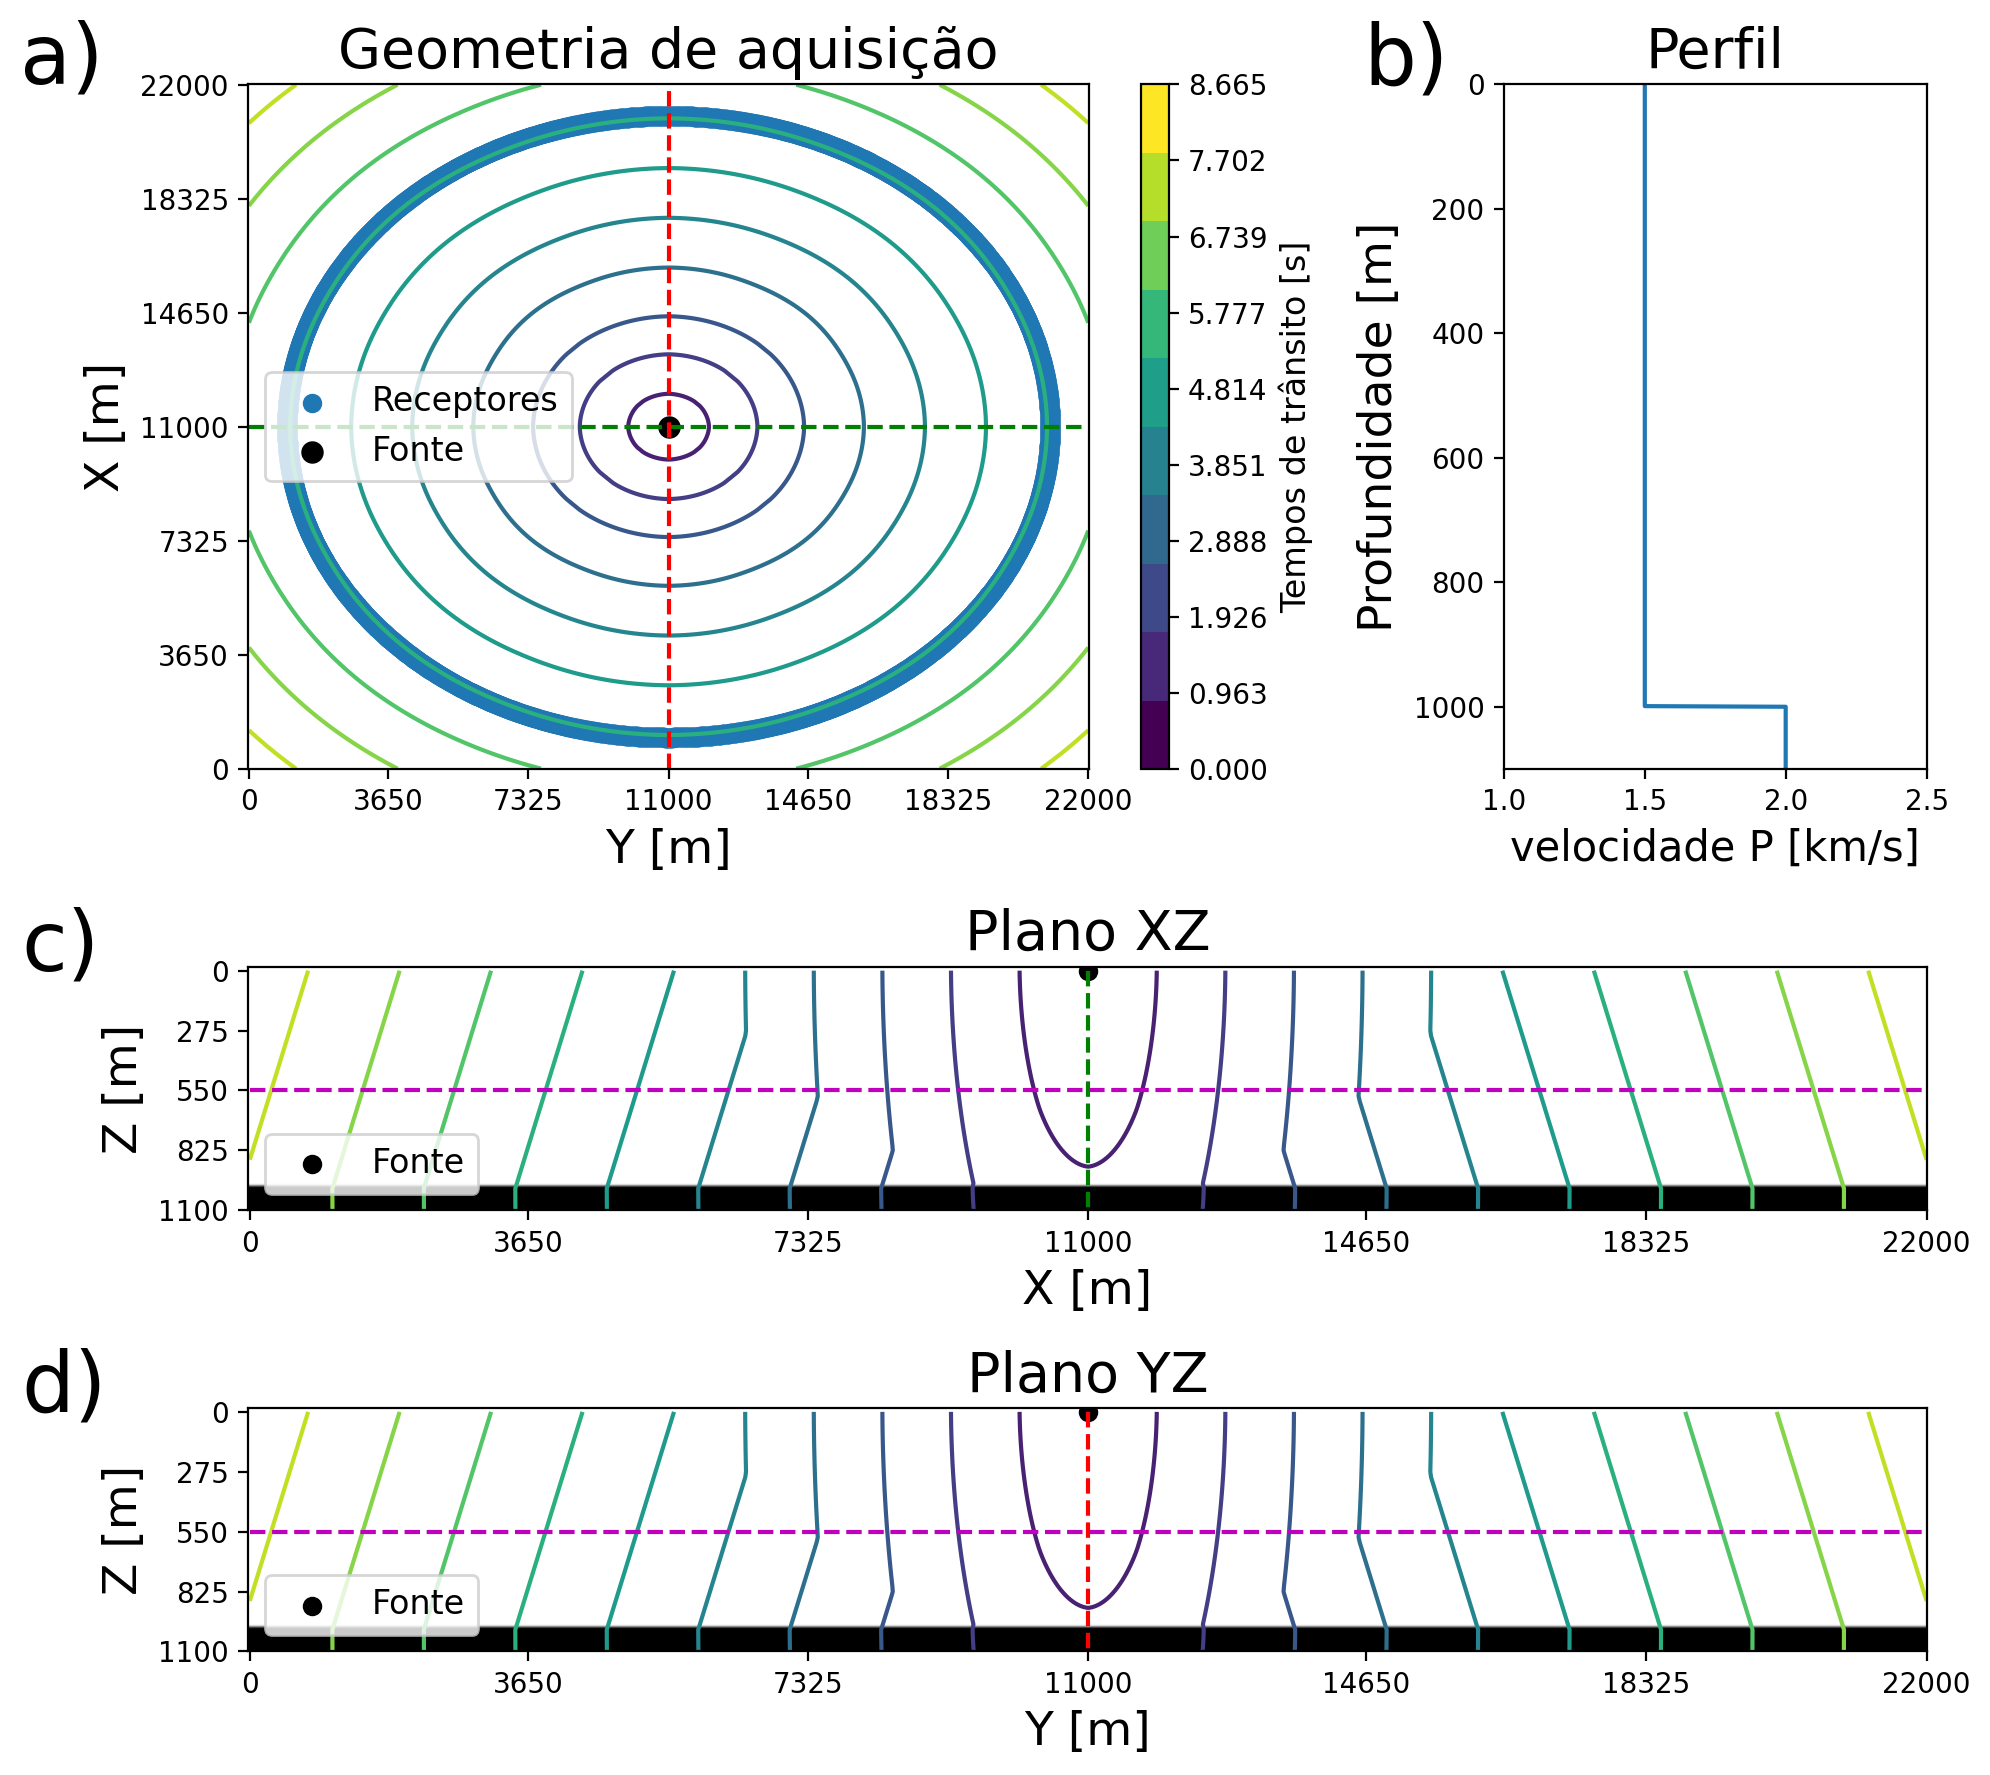
\includegraphics[width = 11cm, height = 10cm]{Imgs/RevisaoBibliografica/modelGeometry.png}
	\caption{Modelo empregado no teste de precisão e performance. (a) Plano XY ilustrando a geometria de aquisição com o arranjo de receptores circulares possuindo somente um tiro central. Isócronas mapeando o comportamento dos tempos de trânsito são mostradas. (b) Perfil de velocidades delimitando a posição da interface. (c) e (d) são as projeções dos cortes em planos XZ e YZ em relação à posição da fonte.}
	\label{fig:configurationNumericalComparison}
\end{figure}


\begin{figure}[H]
	\centering
	\subfloat[]{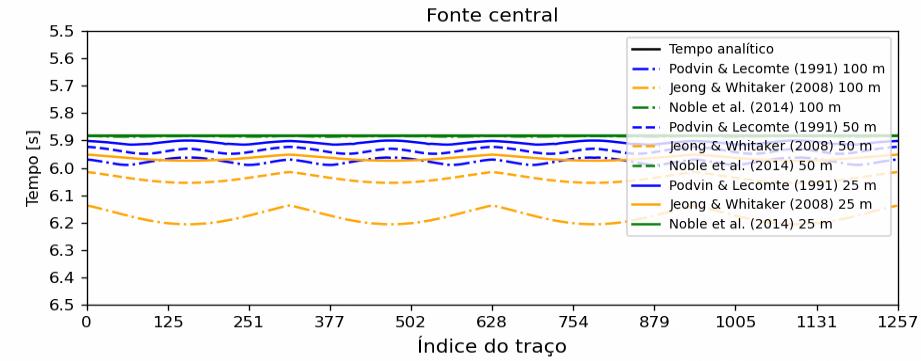
\includegraphics[width=8cm,height=3.5cm]{Imgs/RevisaoBibliografica/precision_direct.png}\label{fig:rnca}}
	\subfloat[]{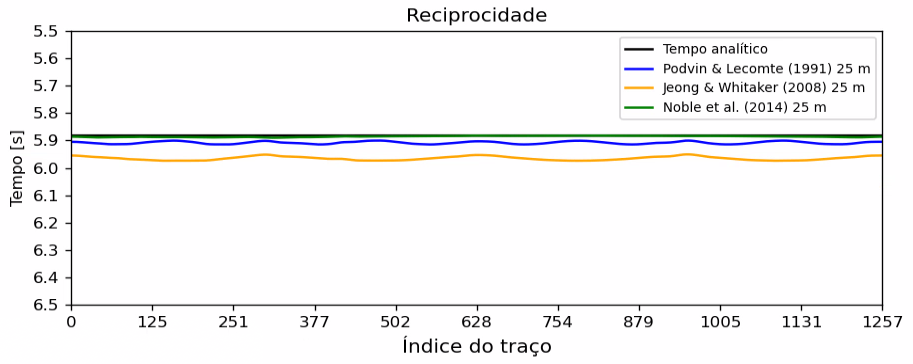
\includegraphics[width=8cm,height=3.5cm]{Imgs/RevisaoBibliografica/reciprocity.png}\label{fig:rncb}}
	
	\subfloat[]{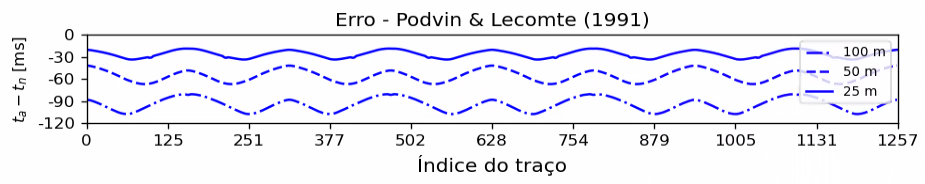
\includegraphics[width=8cm,height=1.5cm]{Imgs/RevisaoBibliografica/error_pod_direct.png}\label{fig:rncc}}
	\subfloat[]{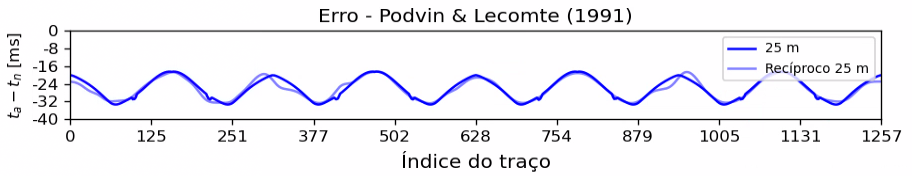
\includegraphics[width=8cm,height=1.5cm]{Imgs/RevisaoBibliografica/error_pod_reciprocity.png}\label{fig:rncd}}
	
	\subfloat[]{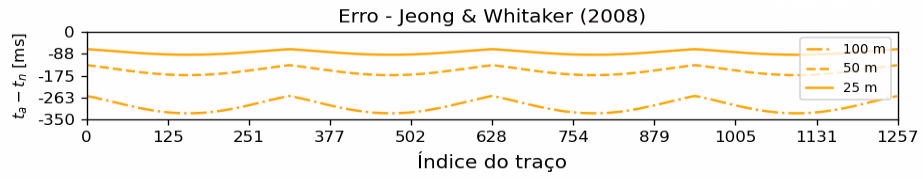
\includegraphics[width=8cm,height=1.5cm]{Imgs/RevisaoBibliografica/error_fim_direct.png}\label{fig:rnce}}
	\subfloat[]{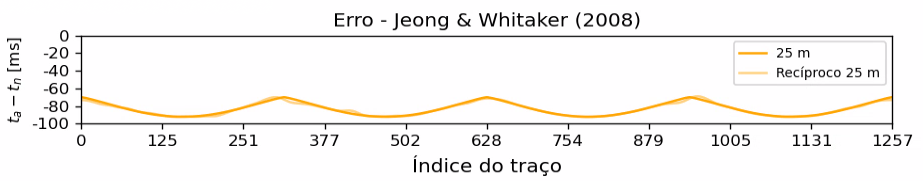
\includegraphics[width=8cm,height=1.5cm]{Imgs/RevisaoBibliografica/error_fim_reciprocity.png}\label{fig:rncf}}
	
	\subfloat[]{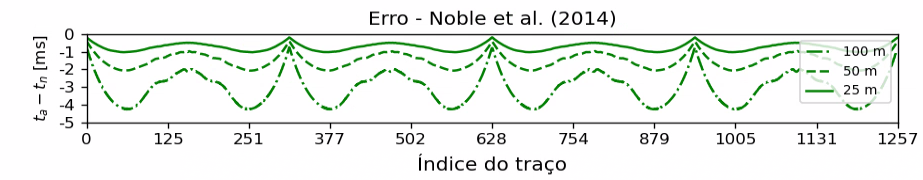
\includegraphics[width=8cm,height=1.5cm]{Imgs/RevisaoBibliografica/error_fsm_direct.png}\label{fig:rncg}}
	\subfloat[]{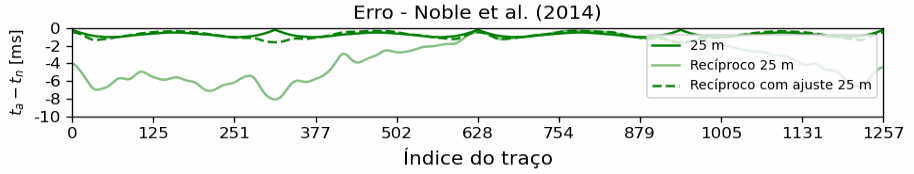
\includegraphics[width=8cm,height=1.5cm]{Imgs/RevisaoBibliografica/error_fsm_reciprocity.png}\label{fig:rnch}}
	
	\caption{Comparação de precisão entre os métodos numéricos estudados. (a) Mapeamento de todas as chegadas para os métodos numéricos testados para os espaçamentos estudados. (b) Estudo de reciprocidade utilizando o espaçamento de 25 m. (c) Escala do erro para as chegadas em diferentes espaçamentos e (d) tempo direto e recíproco utilizando a formulação de \citeonline{podvin1991finite}. (e) Escala do erro e (f) estudo de reciprocidade para a formulação de \citeonline{jeong2008fast}. (g) Escala do erro e (h) estudo de reciprocidade para a formulação de \citeonline{noble2014accurate}.}
	\label{fig:resultsNumericalComparison}
\end{figure}







\section{Inversão tomográfica}

Tipos de tomografia (reflexão, difração, transmissão e refração)







trabalhos do GISIS

\cite{santos2012tomography}
\cite{bulhoes2021efeitos}



teoria de inversão

Função objetivo e linearização

Regularização 

\cite{seo2012nonlinear}
\cite{sain2023active}



least squares conjugate gradient

\cite{saad2003iterative}




\subsection*{Tomografia de refração}

Discretização do modelo

Raios ilustrativos



\subsection*{Obtenção do dado observado}



tipos de picking (manual, analítico, machine learning)

formulação utilizada

\cite{pan2019automatic} 
\cite{qin2021first} 
